%% abtex2-modelo-livro.tex, v-1.9.7 
%% Copyright 2012-2018 by abnTeX2 group at http://www.abntex.net.br/
%%
%% This work may be distributed and/or modified under the
%% conditions of the LaTeX Project Public License, either version 1.3
%% of this license or (at your option) any later version.
%% The latest version of this license is in
%%   http://www.latex-project.org/lppl.txt
%% and version 1.3 or later is part of all distributions of LaTeX
%% version 2005/12/01 or later.
%%
%% This work has the LPPL maintenance status `maintained'.
%%
%% Further information is available on 
%% http://www.abntex.net.br/
%% 


\documentclass[
	% -- opções da classe memoir --
	12pt,				        % tamanho da fonte
	openright,			    % capítulos começam em pág ímpar (insere página vazia caso preciso)
	twoside,			      % para impressão em recto e verso. Oposto a oneside
	a4paper,			      % tamanho do papel. 
	% -- opções da classe abntex2 --
	chapter=TITLE,		  % títulos de capítulos convertidos em letras maiúsculas
	section=TITLE,		  % títulos de seções convertidos em letras maiúsculas
	subsection=TITLE,	  % títulos de subseções convertidos em letras maiúsculas
	subsubsection=TITLE,% títulos de subsubseções convertidos em letras maiúsculas
	% -- opções do pacote babel --
	english,			      % idioma adicional para hifenização
	french,				      % idioma adicional para hifenização
	brazil,				      % o último idioma é o principal do documento
	sumario=tradicional
]{abntex2}


\newcommand\hmmax{0}
\newcommand\bmmax{0}

% compilação de fontes


\usepackage{mathtools}
\usepackage{amsfonts}
\usepackage{mathrsfs} % para mathscr

\usepackage{ifxetex}
\ifxetex
  % % se for utilizar as fontes do sistema: **escolha sua fonte**
    % comandos de fontes
\usepackage{mathspec}
\setmathsfont(Digits,Latin,Greek){Minion Pro}
\setmathrm{Minion Pro}
\setmainfont[Numbers=OldStyle]{Minion Pro} %fonte principal (serifada)
\setsansfont[Scale=0.9]{Myriad Pro} %fonte sem serifas
\setmonofont[Scale=MatchLowercase]{Consolas} % fonte monoespaçada
  
  \usepackage{polyglossia} %always load polyblossia after fonts for digits in math mode
  \setmainlanguage{brazil}
  \setotherlanguages{french,english,spanish,german,italian}  
  
\else
  % % se for utilizar pdflatex
\usepackage[utf8]{inputenc}
%\usepackage{newtxmath} 
%\usepackage{Alegreya}
%\usepackage{AlegreyaSans}
%\usepackage[lf]{FiraMono}
%\usepackage[italic]{mathastext}
\fi

%% Observação: o pacote polyglossia pode apresentar erro ao ser utilizado com ifxetex + babel. 
%% Se isso acontecer, atualize o pacote para a versão mais recente ou utilize somente uma das sequências (pdflatex ou xelatex), comentando ou apagando a outra.

\usepackage{microtype} 				          % para melhorias de justificação
\usepackage[dvipsnames]{xcolor}         % para cores
\usepackage{graphicx} 		            	% para imagens
\usepackage{booktabs,tabularx,rotating}	% para tabelas
\usepackage{mdframed} 				          % para caixas de texto como na CIP do verso do título
\usepackage{multicol}				            % tabelas com colunas mescladas
\usepackage{lettrine}				            % letras capitulares
\usepackage{xspace} 				            % para nao precisar de espaços com {} depois de comandos como \LaTeX e abreviações criadas pelo usuário
\usepackage{lipsum} 				            % para texto de preenchimento de exemplo
\usepackage{leading}				            % espaçamento entrelinhas (leading)
\leading{13pt}
%\usepackage{lmodern}
%\usepackage{gentium}
\usepackage{fouriernc}
%\usepackage{libertine, libertinust1math}
%\usepackage{newpxtext, newpxmath}
%\usepackage[charter]{mathdesign}
%\usepackage[utopia]{mathdesign}
%\usepackage[p,osf,space]{erewhon} % main font
%\usepackage[erewhon,vvarbb,bigdelims]{newtxmath} % math font
\usepackage{amsthm}
\usepackage{multirow,makecell}

% Enumerate
%\usepackage{enumerate}
\usepackage{enumitem}%{shortlabels}

% Correct left and right spacing on math mode
\usepackage{mleftright}

% SI units
\usepackage{siunitx}
\selectlanguage{brazilian}
\sisetup{per-mode=symbol}
\sisetup{exponent-product = \cdot}
\sisetup{retain-explicit-plus}
\sisetup{output-decimal-marker = {,}}
\sisetup{output-complex-root = \jmath}
\sisetup{complex-root-position = before-number}
\sisetup{angle-symbol-degree}

\DeclareSIUnit\atrasado{atrasado}

\DeclareMathOperator{\atan}{atan}

%%%%%%%%%% Barra
\newcommand{\olsi}[1]{\,\overline{\!{#1}}} % overline short italic

%%%%%%%%%% Múltiplas colunas
\usepackage{multicol}
\usepackage{wrapfig}
%\setlength{\columnseprule}{1pt}
%\def\columnseprulecolor{\color{blue}}

%%%%%%%%%% Fórmulas químicas
\usepackage[version=4]{mhchem}
\usepackage{isotope}

% textexamplebox
\usepackage[most]{tcolorbox}
\newcounter{testexample}
\usepackage{xparse}

\def\exampletext{Exemplo} % If English

\NewDocumentEnvironment{testexample}{ O{} }
{
\colorlet{colexam}{black} % Global example color
\newtcolorbox[use counter=testexample]{testexamplebox}{%
    % Example Frame Start
    empty,% Empty previously set parameters
    title={\exampletext\ \thetcbcounter: #1},% use \thetcbcounter to access the testexample counter text
    % Attaching a box requires an overlay
    attach boxed title to top left,
       % Ensures proper line breaking in longer titles
       minipage boxed title,
    % (boxed title style requires an overlay)
    boxed title style={empty,size=minimal,toprule=0pt,top=4pt,left=3mm,overlay={}},
    coltitle=colexam,fonttitle=\bfseries,
    before=\par\medskip\noindent,parbox=false,boxsep=0pt,left=3mm,right=0mm,top=2pt,breakable,pad at break=0mm,
       before upper=\csname @totalleftmargin\endcsname0pt, % Use instead of parbox=true. This ensures parskip is inherited by box.
    % Handles box when it exists on one page only
    overlay unbroken={\draw[colexam,line width=.5pt] ([xshift=-0pt]title.north west) -- ([xshift=-0pt]frame.south west); },
    % Handles multipage box: first page
    overlay first={\draw[colexam,line width=.5pt] ([xshift=-0pt]title.north west) -- ([xshift=-0pt]frame.south west); },
    % Handles multipage box: middle page
    overlay middle={\draw[colexam,line width=.5pt] ([xshift=-0pt]frame.north west) -- ([xshift=-0pt]frame.south west); },
    % Handles multipage box: last page
    overlay last={\draw[colexam,line width=.5pt] ([xshift=-0pt]frame.north west) -- ([xshift=-0pt]frame.south west); },%
    }
\begin{testexamplebox}}
{\end{testexamplebox}\endlist}

%%%%%%%%%% big cdot
\makeatletter
\newcommand*\bigcdot{\mathpalette\bigcdot@{1}}
\newcommand*\bigcdot@[2]{\mathbin{\vcenter{\hbox{\scalebox{#2}{$\m@th#1\bullet$}}}}}
\makeatother

%%%%%%%%%% \oint
\usepackage{esint}

%%%%%%%%%% phase for complex
\usepackage{steinmetz}

% pgfplots
\usepackage{pgfplots}
\pgfplotsset{compat=newest}

% tikz
\usepackage{textpos}
\usepackage{tikz}
\usepackage{tikz-3dplot}
\usetikzlibrary{arrows.meta,calc,decorations.markings,math,arrows.meta,bending,shapes.geometric,shapes.symbols,patterns}
\usetikzlibrary{intersections, pgfplots.fillbetween}

%%%%%%%%%% Citar múltiplas equações
\usepackage[brazilian]{cleveref}

%%%%%%%%%% Math in bold
\usepackage{bm}

\def\shrug{\texttt{\raisebox{0.75em}{\char`\_}\char`\\\char`\_\kern-0.5ex(\kern-0.25ex\raisebox{0.25ex}{\rotatebox{45}{\raisebox{-.75ex}"\kern-1.5ex\rotatebox{-90})}}\kern-0.5ex)\kern-0.5ex\char`\_/\raisebox{0.75em}{\char`\_}}}

% tikz
\usepackage{tikz}
\usepackage{pgfplots}
\usepackage[american,RPvoltages]{circuitikz}
\usetikzlibrary{babel,arrows.meta,calc,decorations.markings,math,arrows.meta,bending}
\usetikzlibrary{intersections, pgfplots.fillbetween}

% Subfigure
%\makeatletter
%\let\normalsize\relax
%\let\@currsize\normalsize
%\makeatother
\usepackage{caption}
\usepackage{subcaption}
%\usepackage{setspace}

% ---
% Pacotes de citações
% ---
\usepackage[brazilian,hyperpageref]{backref}	 % Paginas com as citações na bibl
\usepackage[alf]{abntex2cite}	% Citações padrão ABNT

% ---
% Configurações do pacote backref
% Usado sem a opção hyperpageref de backref
\renewcommand{\backrefpagesname}{Citado na(s) página(s):~}
% Texto padrão antes do número das páginas
\renewcommand{\backref}{}
% Define os textos da citação
\renewcommand*{\backrefalt}[4]{
	\ifcase #1 %
		Nenhuma citação no texto.%
	\or
		Citado na página #2.%
	\else
		Citado #1 vezes nas páginas #2.%
	\fi}%
% ---

% ---
% Informações do documento
% ---
\titulo{Título bem bonito}
\autor{Huguinho \and Zézinho \and Luísinho}
\data{\num{2024}, v-1.0}
\preambulo{Resumo do que se trata esse material}
\local{São José dos Campos}
\instituicao{Instituto Federal de São Paulo.\\ \emph{Campus} São José dos Campos}

% alterando o aspecto da cor azul
\definecolor{blue}{RGB}{41,5,195}

% informações do PDF
\makeatletter
\hypersetup{
     	%pagebackref=true,
		pdftitle={\@title}, 
		pdfauthor={\@author},
    	pdfsubject={\imprimirpreambulo},
	    pdfcreator={LaTeX with abnTeX2},
		pdfkeywords={abnt}{latex}{abntex}{abntex2}{livro}, 
		colorlinks=true,       		% false: boxed links; true: colored links
    	linkcolor=blue,          	% color of internal links
    	citecolor=blue,        		% color of links to bibliography
    	filecolor=magenta,      		% color of file links
		urlcolor=blue,
		bookmarksdepth=4
}
\makeatother
% ---


% ---
% Estilo de capítulos
%
%\chapterstyle{pedersen} 
%\chapterstyle{lyhne} 
%\chapterstyle{madsen} 
\chapterstyle{veelo} 
%
% Veja outros estilos em:
% https://www.ctan.org/tex-archive/info/MemoirChapStyles
% ---

% para cabeçalhos sem estar em maiúsculas
%\nouppercaseheads 

% -----
% Declarações de cabecalhos 
% -----
% Cabecalho padrao
\makepagestyle{abntbookheadings}
\makeevenhead{abntbookheadings}{\ABNTEXfontereduzida\thepage}{}{\ABNTEXfontereduzida\textit\leftmark}
\makeoddhead{abntbookheadings}{\ABNTEXfontereduzida\textit\rightmark}{}{\ABNTEXfontereduzida\thepage}
\makeheadrule{abntbookheadings}{\textwidth}{\normalrulethickness}

% Cabecalho do inicio do capitulo
\makepagestyle{abntbookchapfirst}
\makeoddhead{abntbookchapfirst}{}{}{}

% Configura layout para elementos textuais
\renewcommand{\textual}{%
  \pagestyle{abntbookheadings}%
  \aliaspagestyle{chapter}{abntbookchapfirst}% customizing chapter pagestyle
  \nouppercaseheads%
  \bookmarksetup{startatroot}% 
}
% ---

% Margens do documento 
%% (margens do abntex2 não combinam nem com A5 nem com estilos de capítulo da
% classe memoir.)
\setlrmarginsandblock{2.5cm}{3.5cm}{*}
\setulmarginsandblock{2.5cm}{3.5cm}{*}
\checkandfixthelayout
% ---


% ---
% Início do documento
% ---
\begin{document}
\frenchspacing

\frontmatter

% ---
% Capa principal
% ---
\begin{titlingpage}
\phantom{xxx}
\vspace{0.5cm}
\huge
\raggedright
\imprimirautor\\
\vspace{2.5cm}
\huge 
{\raggedleft

\includegraphics[scale=1]{Figuras/Marca_IFSP_2015_SaoJosedosCampos-01}\\[1cm]
\textit{\textcolor{blue}{\imprimirtitulo}}\\[1cm]
}
\centering 
% %este é um símbolo que só aparecerá com a fonte Minion.
\vfill
\Large
% %este é um símbolo que só aparecerá com a fonte Minion.
\imprimirinstituicao
\end{titlingpage}
% ---

% ---
% Contra-capa
% ---
\begin{titlingpage}

\phantom{xxx}
\vspace{0.5cm}
\huge
\raggedright
\imprimirautor\\
\vspace{2.5cm}
\huge 
{\raggedleft

\includegraphics[scale=1]{Figuras/Marca_IFSP_2015_SaoJosedosCampos-02}\\[1cm]
\textit{\textcolor{blue}{\imprimirtitulo}}\\[1cm]
}
\centering 
% %este é um símbolo que só aparecerá com a fonte Minion.
\vfill
\Large
% %este é um símbolo que só aparecerá com a fonte Minion.
\imprimirinstituicao
% ---

% ---
% Verso da contra-capa
% ---
\clearpage
\ABNTEXfontereduzida
%\raggedright
© 2023 \imprimirautor \space \& \imprimirinstituicao
%este é só um exemplo de copyright.

Qualquer parte desta publicação pode ser reproduzida, desde que citada a fonte.

\vspace*{\fill}

\begin{center}
Dados Internacionais de Catalogação na Publicação (\textsc{cip})
Câmara Brasileira do Livro, \textsc{sp}, Brasil
\end{center}

\begin{mdframed}
\noindent Tal, Fulano de.

\imprimirtitulo. / \imprimirautor. -- \imprimirlocal: \imprimirinstituicao
Ltda., \num{2024}.

\medskip

Bibliografia.

ISBN XXXX-XXXX-XX.

\medskip

1. Programas de computador. 2. Tipografia. 3. Latex. 4. Normas ABNT.

\end{mdframed}

\end{titlingpage}
% ---

% ---
% inserir lista de ilustrações
% ---
\pdfbookmark[0]{\listfigurename}{lof}
\listoffigures*
\cleardoublepage

% ---
% inserir lista de tabelas
% ---
\pdfbookmark[0]{\listtablename}{lot}
\listoftables*
\cleardoublepage
% ---

% ---
% inserir o sumario
% ---
\pdfbookmark[0]{\contentsname}{toc}
\tableofcontents*
\cleardoublepage
% ---

% ------------------------------------------------------------
% Início da parte textual
% ------------------------------------------------------------
%\textual
\mainmatter
% ------------------------------------------------------------

% ------------------------------------------------------------
\part[Eletrostática]{Eletrostática}
% ------------------------------------------------------------

% ------------------------------------------------------------
\chapter[Eletrização]{Eletrização}
% ------------------------------------------------------------

%%%%%%%%%%%%%%%%%%%%%%%%%%%%%%%%%%%%%%%%%%%%%%%%%%%%%%%%%%%%%%%%%%%%%%%%%%%%%%%%%%%%%%%%%%%%%%%%%%%%
\section{Introdução}
%%%%%%%%%%%%%%%%%%%%%%%%%%%%%%%%%%%%%%%%%%%%%%%%%%%%%%%%%%%%%%%%%%%%%%%%%%%%%%%%%%%%%%%%%%%%%%%%%%%%

O termo \textbf{escalar} refere-se a uma quantidade cujo valor pode ser representado por um único número real (positivo ou negativo). Os $x$, $y$ e $z$ que usamos na álgebra básica são escalares, assim como as quantidades que eles representam. Se falamos de um corpo caindo uma distância $L$ em um tempo $t$, ou a temperatura $T$ em qualquer ponto cujas coordenadas são $x$, $y$ e $z$, então $L$, $t$, $T$, $x$, $y$ e $z$ são todos escalares. Outras grandezas escalares são massa, densidade, pressão (mas não força), volume, resistividade de volume e tensão.

Uma grandeza \textbf{vetorial} tem módulo e direção no espaço. Adotamos a convenção de que magnitude infere valor absoluto; a magnitude de qualquer quantidade é, portanto, sempre positiva. Estamos preocupados apenas com espaços bidimensionais e tridimensionais, mas os vetores podem ser definidos no espaço $n$-dimensional em aplicações mais avançadas. Força, velocidade, aceleração e uma linha reta do terminal positivo ao negativo de uma bateria de armazenamento são exemplos de vetores. Cada quantidade é caracterizada por uma magnitude e uma direção.

%%%%%%%%%%%%%%%%%%%%%%%%%%%%%%%%%%%%%%%%%%%%%%%%%%%%%%%%%%%%%%%%%%%%%%%%%%%%%%%%%%%%%%%%%%%%%%%%%%%%
\subsection{Adição e subtração}

A adição de vetores segue a lei do paralelogramo. A \cref{fig:01p01} mostra a soma de dois vetores, $\bm{\vec{A}}$ e $\bm{\vec{B}}$. É fácil ver que $\bm{\vec{A}} + \bm{\vec{B}} = \bm{\vec{B}} + \bm{\vec{A}}$, ou que a adição de vetores obedece à lei comutativa. A adição vetorial também obedece à lei associativa,
\begin{align*}
	\bm{\vec{A}} + \left( \bm{\vec{B}} + \bm{\vec{C}} \right) = \left( \bm{\vec{A}} + \bm{\vec{B}} \right) + \bm{\vec{C}}
\end{align*}

\begin{figure}
	\centering
	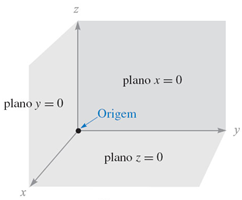
\includegraphics[width=\linewidth]{Figuras/Fig01p02a}
	\caption{Sistema de coordenadas retangulares do tipo triedro direito. Se os dedos curvados da mão direita indicam a direção pela qual o eixo $x$ deve ser girado para coincidir com o eixo $y$, o polegar mostra a direção do eixo $z$.}
	\label{fig:01p02}
\end{figure}
% ------------------------------------------------------------
\postextual % pós-textual
% ------------------------------------------------------------


% ------------------------------------------------------------
%\bibliography{Refs} % insere o arquivo de bibliografia


% ------------------------------------------------------------

% ------------------------------------------------------------
% Inicia os apêndices
% ------------------------------------------------------------
\begin{apendicesenv}

% Imprime uma página indicando o início dos apêndices
\partapendices

% ----------------------------------------------------------
\chapter{Respostas dos problemas}
% ----------------------------------------------------------

\section*{Sistemas elétricos de potência: um cenário em transformação}

\begin{multicols}{2}
\begin{enumerate}[label=\arabic*.,start=1]

%%%%%%%%%% 01
	\item Essa é com você

%%%%%%%%%% 02
	\item Essa é com você
	
%%%%%%%%%% 03
	\item Essa é com você
	
%%%%%%%%%% 04
	\item Essa é com você
	
	
\end{enumerate}
\end{multicols}

\end{apendicesenv}
% ---

% ------------------------------------------------------------
% Colofão: última página com informações sobre a composição do livro.
\cleardoublepage
\thispagestyle{empty} 

\end{document}
